\chapter{Strumenti}
Per analizzare le varie architetture presentate dobbiamo prima fare un discorso sugli strumenti utilizzati per costruire una applicazione web e che useremo per gli esempi di codice dei capitoli successivi.

\section{ECMAScript 2015}
Anche conosciuto come \textit{ECMAScript6}\footnote{https://www.ecma-international.org/ecma-262/6.0}, è una standardizzazione del linguaggio Javascript creata da Ecma International. Questa versione in particolare mette a disposizione features molto utili per scrivere codice che si avvicina al paradigma di programmazione funzionale. Possiamo classificare ECMAScript come un linguaggio a sé e differente da Javascript, che in principio doveva essere utilizzato solamente come linguaggio di scripting lato client, ma che ora viene utilizzato come vero e proprio linguaggio di programmazione su ambienti e scale differenti.
 
Quando si parla di applicazioni web, e più in particolare del loro front-end, ci si riferisce tuttavia a quel codice Javascript che viene scaricato ed interpretato dal browser dell'utente. Sorge quindi il serio problema di far eseguire un codice su una macchina il cui interprete potrebbe non supportarlo a dovere, ad esempio nel caso in cui si utilizzi ES6 in un browser che supporta solo uno standard più vecchio. Proprio per questo si utilizzano strumenti come \textit{Babel}\footnote{https://babeljs.io} che hanno la funzione di \textit{transpiler}, ossia di compilare codice sorgente Javascript da uno standard nuovo e poco supportato ad ECMAScript5 (o inferiore) che è implementato dalla stragrande maggioranza dei browser.

Le funzionalità introdotte da ECMAScript6 sono molte, tuttavia qui parleremo solo di quelle che risulteranno propedeutiche per capire il codice dei capitoli successivi.

\subsection{Let e Const}
Una delle features introdotte, che probabilmente è anche una delle più incisive, riguarda l'assegnazione delle variabili. In ES5 la dichiarazione avveniva tramite la keyword \textit{var} ed il loro scope era relativo alla funzione direttamente loro superiore (Codice \ref{exampleVarES5}). E' bene notare che questi tipi di variabili sono legate al contesto (e quindi alla funzione) dove sono definite e non al blocco di codice \mintinline{text}{{ /* ... */ }} in cui sono dichiarate, a differenza di molti altri linguaggi di programmazione.
 
\begin{listing}[ht]
\inputminted{Javascript}{sources/exampleVarES5.js}
\caption{Esempio della dichiarazione di una variabile con \textit{var}.}
\label{exampleVarES5}
\end{listing}

In ES6 a questa si aggiungono anche \text{let} e \textit{const} il cui scope è relativo al blocco in cui sono posizionate (e non alla funzione, come in \textit{var}). La prima non ha nulla di particolare oltre ciò che abbiamo già detto, la seconda invece dichiara variabili costanti, ossia il cui valore non può mutare attraverso una riassegnazione e non possono essere ridichiarate (Codice \ref{exampleLetConstES6}).

\begin{listing}[ht]
\inputminted{Javascript}{sources/exampleLetConstES6.js}
\caption{Esempio della dichiarazione di variabili con \textit{let} e \textit{const}.}
\label{exampleLetConstES6}
\end{listing}

La keyword \textit{const} verrà molto utilizzata nei successivi codici in quanto permette di utilizzare un concetto fondamentale dei linguaggi funzionali: l'immutabilità\footnote{Il concetto di immutabilità è un pilastro fondamentale della programmazione funzionale. Avere un elemento immutabile significa che l'unico modo per modificarlo è quello di crearne uno nuovo con le modifiche volute e modificare la referenza a quest'ultimo.}, oltre al fatto che utilizzare delle variabili non mutabili riduce il rischio di errori e semplifica il debugging del codice.

\subsection{Arrow Function}
In Javascript la parola chiave \textit{this} si riferisce al contesto dove viene eseguita. Può essere in parte paragonata al modo in cui nella programmazione ad oggetti ci si riferisce all'istanza su cui stiamo lavorando. La grossa differenza tuttavia è che in Javascript cambiare il contesto e quindi avere un valore del \textit{this} inaspettato è estremamente semplice e comporta non poche problematiche nell'analisi di un codice.

\begin{listing}[ht]
\inputminted{Javascript}{sources/exampleShadowThisES5.js}
\caption{Esempio di comportamento inaspettato di \textit{this}.}
\label{exampleShadowThisES5}
\end{listing}

Si consideri il Codice \ref{exampleShadowThisES5}. Il problema illustrato si verifica perché il contesto dove viene eseguito il \textit{this} non è più quello dell'oggetto \textit{Foo}, ma un contesto separato ristretto alla funzione \textit{setInterval}. Per evitare problemi di questo genere (che ovviamente non sono relativi solo alla funzione \textit{setInterval} ma ad un vasto numero di altri casi particolari) ES6 mette a disposizione le \textit{Arrow Function}, ossia funzioni anonime sintatticamente più corte che non sovrascrivono il \textit{this} del contesto precedente permettendo la scrittura di un codice ad oggetti più sicuro e senza comportamenti inaspettati (Codice \ref{exampleArrowFunctionES6}).

\begin{listing}[ht]
\inputminted{Javascript}{sources/exampleArrowFunctionES6.js}
\caption{Esempio di \textit{Arrow Function}.}
\label{exampleArrowFunctionES6}
\end{listing} 

\subsection{Parametri predefiniti e ad oggetti}
ES6 permette di utilizzare valori predefiniti per i parametri delle funzioni che creiamo. Questi valori di default vengono assegnati quando i normali parametri sono \textit{undefined} (Codice \ref{exampleDefaultParametersES6}). 

\begin{listing}[ht]
\inputminted{Javascript}{sources/exampleDefaultParametersES6.js}
\caption{Esempio di utilizzo dei parametri di default.}
\label{exampleDefaultParametersES6}
\end{listing}

Un altro miglioramento apportato da ES6 riguarda gli oggetti passati come parametri. E' ora possibile destrutturare un oggetto direttamente dai parametri durante la definizione di una funzione (Codice \ref{exampleObjectParameterES6}).

\begin{listing}[ht]
\inputminted{Javascript}{sources/exampleObjectParameterES6.js}
\caption{Esempio di destrutturazione di un oggetto passato come parametro.}
\label{exampleObjectParameterES6}
\end{listing}

\subsection{Classi}
In Javascript non esistono classi ma esistono invece oggetti con proprietà particolari che ci permettono di simulare ereditarietà e riusabilità. ES5 non possiede una vera e propria parola chiave per definire una classe, e quindi per creare un oggetto che si comporti come tale partiamo dal costruttore per poi aggiungere i metodi voluti (Codice \ref{examplePrototypeInheritanceES5}). Questa tecnica prende il nome di Prototypal Inheritance \cite{RylanOnPrototypeInheritance}.

\begin{listing}[ht]
\inputminted{Javascript}{sources/examplePrototypeInheritanceES5.js}
\caption{Esempio di una classe in ES5.}
\label{examplePrototypeInheritanceES5}
\end{listing}

ES6 mette a disposizione una sintassi molto più comprensibile e versatile per la gestione delle classi che rimane però solamente un abbellimento sopra il concetto di Prototypal Inheritance (Codice \ref{exampleClassES6}). 

\begin{listing}[ht]
\inputminted{Javascript}{sources/exampleClassES6.js}
\caption{Esempio di una classe in ES6.}
\label{exampleClassES6}
\end{listing}

\subsection{Struttura statica dei moduli}
\label{strutturaStaticaDeiModuli}
Un modulo in Javascript corrisponde ad un'unità autonoma dell'applicazione che contiene tutto il necessario per eseguire una particolare e distinta funzionalità di questa. La struttura dei moduli di ES5, usando ad esempio la sintassi di \textit{CommonJS}\footnote{http://requirejs.org/docs/commonjs.html}, è dinamica ciò significa che l'importazione e l'esportazione è mutabile a seconda dell'esecuzione del codice ed avviene quindi a run-time (Codice \ref{exampleDynamicImportES5}). Questo comporta che per analizzare le dipendenze di un progetto ed eliminare eventuali elementi non utilizzati, sia necessario eseguire il codice e monitorarne il comportamento in quanto non sappiamo a priori quali importazioni ed esportazioni verranno eseguite.

\begin{listing}[ht]
\inputminted{Javascript}{sources/exampleDynamicImportES5.js}
\caption{Esempio di importazione dinamica di un modulo in ES5.} 
\label{exampleDynamicImportES5}
\end{listing}

ES6 mette a disposizione un sistema di gestione dei moduli statico (Codice \ref{exampleImportExportES6}). Questo comporta la possibilità di analizzare le dipendenze di un codice a compile-time in quanto non sono presenti elementi dinamici che obbligano l'esecuzione del codice, con la conseguenza quindi di poter eliminare tutto ciò che non viene effettivamente utilizzato senza eseguire una singola riga di Javascript.
Ovviamente in questo caso non è più possibile posizionare l'importazione o l'esportazione di un modulo all'interno di un costrutto o utilizzare variabili.

\begin{listing}[ht]
\inputminted{Javascript}{sources/exampleImportExportES6.js}
\caption{Esempio di importazione statica di un modulo in ES6.} 
\label{exampleImportExportES6} 
\end{listing}

\section{Webpack}
Abbiamo parlato nella sezione precedente di Webpack\footnote{https://webpack.js.org} e di come è in grado di trasformare ECMAScript 6 nella sua precedente versione supportata da quasi tutti i browser attuali. Tuttavia questa è solo una piccola caratteristica rispetto a quello che è veramente.
Nel sito ufficiale Webpack è descritto come \blockquote{A module bundler for modern JavaScript applications}. In pratica si occupa di ricercare tutte le dipendenze dell'applicazione e raggrupparle in file aggregati. 
Per capire appieno questo concetto è bene analizzare la struttura di una applicazione Javascript moderna che normalmente consideriamo divisa in due parti ben distinte: il codice sorgente di base e i moduli (sia propri che di terzi) che implementano le varie funzioni. Come abbiamo detto nella Sezione \ref{strutturaStaticaDeiModuli}, un modulo è un'unità autonoma dell'applicazione che ne rappresenta una funzionalità distinta. Un modulo può includere dentro di sé una o più librerie, ossia delle collezioni di funzioni e metodi per risolvere dei particolari problemi. Quello che fa Webpack è analizzare il file Javascript relativo alla nostra applicazione, chiamato “Entry point", e creare un pacchetto con tutti i moduli e le librerie richieste affinché il servizio possa funzionare in maniera corretta (Figura \ref{webpackWorkflow}). 

\begin{figure}[h]
\centering
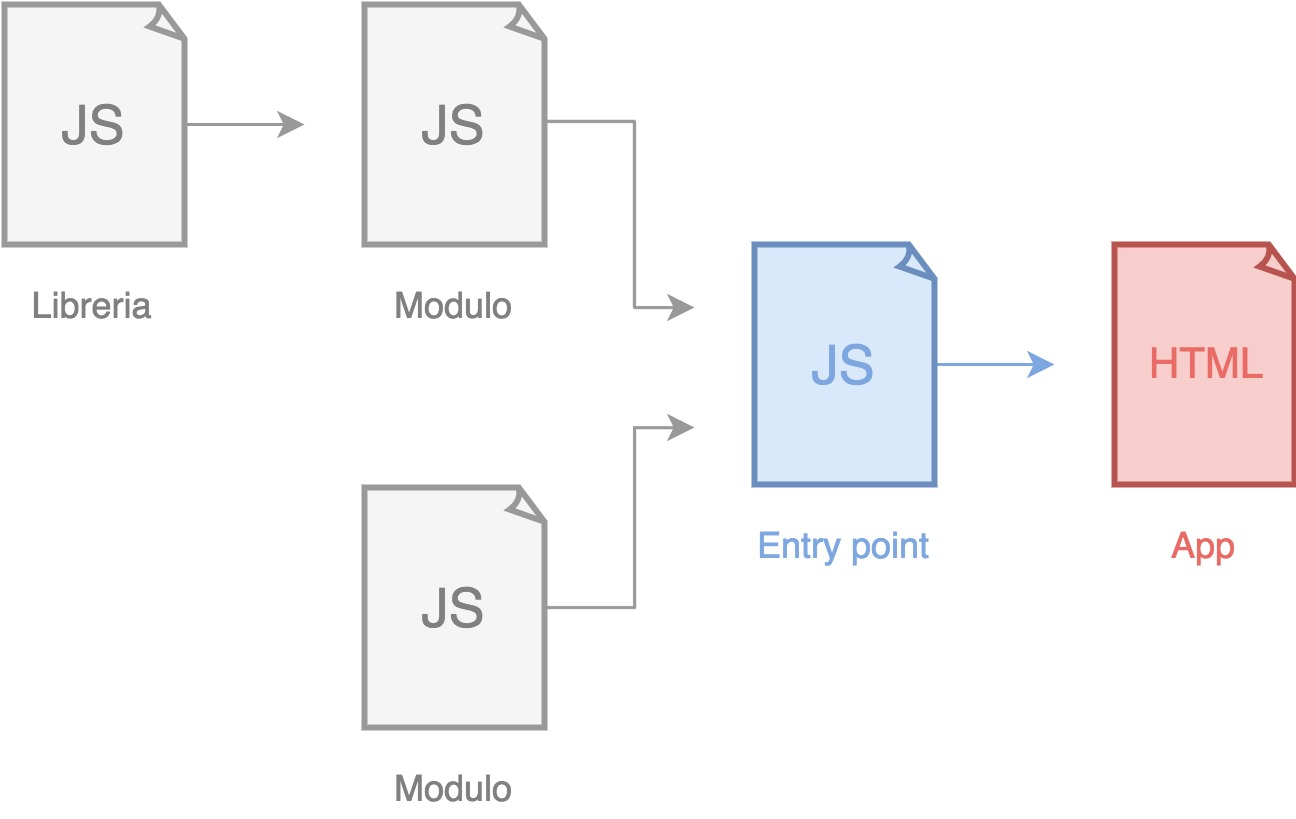
\includegraphics[width=9cm]{./images/webpackWorkflow}
\caption{Rappresentazione del sistema di impacchettamento di Webpack.}
\label{webpackWorkflow}
\end{figure}

Con Webpack diventa estremamente facile suddividere l'applicazione in file di dipendenze multipli che possono includere da codici sorgenti come moduli Javascript o CSS, fino ad immagini e font.
E' anche possibile utilizzare \textit{Loader}, ossia dei middleware, che prendono in input delle dipendenze specifiche e le trasformano a seconda di ciò che abbiamo bisogno (Il transpiler da ES6 ad ES5 fa esattamente questo prendendo in input ogni file Javascript).

\subsection{Hot Module Replacement}
Un aspetto molto interessante di Webpack riguarda l'\textit{Hot Module Replacement} (HMR) che si occupa di aggiungere o rimuovere i pacchetti di dipendenze generati nel run-time dell'applicazione senza un aggiornamento completo della pagina. Questo è molto utile in fase di development in quanto consente di mantenere lo stato di una applicazione anche dopo aver effettuato modifiche al sorgente ed avere le nuove caratteristiche disponibili in maniera molto più veloce del normale aggiornando solo ciò che è necessario. 



\subsection{Tree Shaking}
La tecnica del \textit{Tree Shaking} permette di eliminare il codice inutilizzato all'interno della codebase. Quello che fa Webpack è andare ad analizzare la struttura di \textit{Import} ed \textit{Export} del sorgente che, come abbiamo detto precedentemente nella sezione riguardante ES6, è statica ossia è possibile analizzarla a \textit{compile-time} senza la necessità di eseguire il codice. Una volta trovati gli elementi che non vengono utilizzati essi vengono classificati come “codice morto" e vengono marcati attraverso adeguati commenti. Webpack non si occupa di eliminare questi elementi ma affida il compito ad un eventuale \textit{Minifier} (come ad esempio \textit{UglifyJS}\footnote{https://github.com/mishoo/UglifyJS}) che si occupa di ottimizzare il codice Javascript.

\section{React}
\label{ReactExplanation}
React è una libreria scritta ed utilizzata da Facebook per la creazione di interfacce utente interattive in maniera funzionale ed altamente scalabile che fa uso di diverse tecnologie all'avanguardia come il \textit{Virtual DOM} ed il \textit{Server-side Rendering} \cite{WheelerOnReact}. 
Si basa sul concetto di “componente” come elemento base fondamentale che permette di dividere l'interfaccia in pezzi autonomi e riutilizzabili.
Un componente non è altro che una funzione Javascript che accetta delle proprietà arbitrarie (solitamente chiamate “props”) e ritorna un elemento React generalmente descritto tramite codice JSX, un'astrazione sopra il normale DOM. Un componente può anche essere definito estendendo la classe \mintinline{text}{React.Component}, ottenendo diverse funzionalità aggiuntive come eventi sul suo ciclo di vita e gestione del suo stato interno. Il concetto funzionale di composizione si adatta benissimo a React: un componente complesso dovrebbe essere formato da componenti più piccoli e agnostici che possono quindi essere riutilizzati in altri componenti complessi (Codice \ref{exampleReactComponents}).

\begin{listing}[ht]
\inputminted{jsx}{sources/exampleReactComponents.js}
\caption{Esempio di composizione tra componenti React.}
\label{exampleReactComponents}
\end{listing}

Un pattern molto utilizzato quando si scrive componenti React consiste nel suddividere questi in due categorie fondamentali: \textit{Componenti di presentazione} e \textit{Componenti contenitori}. I primi sono classificati come componenti senza stato interno (\textit{Stateless components}), definiscono lo stile degli elementi, sono estremamente riutilizzabili e non dipendono direttamente dalla logica dell'applicazione ma dalle proprietà ottenute dai componenti superiori di cui fanno parte. Un esempio di componente di presentazione potrebbe essere un bottone, un campo di testo, o una lista.
I componenti contenitori invece sono incaricati di gestire la logica dell'applicazione e forniscono i dati e gli eventi ai componenti di presentazione. Questo approccio migliora la separazione delle occupazioni all'interno dell'interfaccia definendo i componenti contenitori come dei super-componenti con uno stato interno ed un ruolo attivo nell'architettura dell'applicazione che si compongono attraverso i vari componenti di presentazione autonomi.

\subsection{Virtual DOM}
Il  \textit{Document Object Model} (DOM) è una API che definisce la struttura di un documento HTML e come essa viene acceduta e manipolata. E' una rappresentazione ad oggetti di una pagina web la quale può essere modificata con un linguaggio di scripting come Javascript.
Per fare un esempio pratico, lo standard DOM stabilisce che l'interfaccia \textit{Document} rappresenti l'intera pagina HTML e che concettualmente sia il nodo root. L'interfaccia \textit{Node} rappresenta invece l'elemento base ossia il singolo nodo all'interno di un documento e l'implementazione di questa richiede la creazione dei metodi per la gestione del nodo stesso e dei propri figli \cite{HWRWhatIsDOM}.

Quando parliamo di Virtual DOM parliamo di un'astrazione sopra l'astrazione del DOM (Figura \ref{virtualDOMWorkflow}). Modificare quest'ultimo non è particolarmente dispendioso (si tratta solamente di modificare un oggetto Javascript); è tuttavia il processo di lettura e di “ridisegno" della pagina da parte del browser il vero problema. Questa tecnologia riesce a risolvere il suddetto problema mantenendo in memoria una rappresentazione del DOM reale che utilizza il design pattern \textit{Observer}\footnote{Il design pattern Observer si compone di un oggetto chiamato “Subject" che mantiene una lista di altri oggetti dipendenti chiamati "Observers" e li notifica ogni qualvolta il suo stato viene modificato.} per capire quale particolare nodo è stato modificato generando successivamente un nuovo albero derivato dal precedente ma con il nuovo stato. A questo punto effettua complessi algoritmi di differenza per trovare il numero minimo di passaggi per aggiornare il DOM reale per poter infine effettuare la riconciliazione \cite{MishraOnVirtualDOM}.

Il concetto che permette al Virtual DOM di garantire prestazioni maggiori sul DOM reale consiste nell'aggiornamento aggregato. Tutti i cambiamenti effettuati da un evento (che sono i passaggi trovati dall'algoritmo di differenza) vengono aggregati ed il DOM viene ridisegnato solamente una volta.

\begin{figure}[h]
\centering 
\vspace*{0.5cm}

\includegraphics[width=13cm]{./images/virtualDOMWorkflow}
\caption{Posizione del Virtual DOM all'interno di una applicazione React.}
\label{virtualDOMWorkflow}
\vspace*{0.5cm}
\end{figure}

React implementa il Virtual DOM attraverso \textit{JSX}, una estensione di ECMAScript simile ad XML che permette di scrivere elementi di markup con una sintassi simile all'HTML all'interno dei componenti dell'interfaccia. Portare l'HTML all'interno del codice sorgente Javascript offre dei vantaggi non banali come ad esempio il debugging compile-time degli errori di sintassi durante la costruzione del DOM, la versatilità di avere un linguaggio di scripting per effettuare composizione ed altre azioni dinamiche e sopratutto avere una perfetta separazione tra componenti differenti.

\subsection{Server-side rendering}
\label{ReactServerSideRendering}
React è una libreria \textit{isomorfica}, cioè è in grado di essere eseguita sia lato client che lato server. Essa trae vantaggio da NodeJS ed dal fatto che il principale linguaggio di programmazione per entrambi gli ambienti sia sempre Javascript.
Il vantaggio di eseguire React anche lato server risiede nella prima visualizzazione. In una SPA normale durante il primo caricamento vengono scaricati gli elementi base per la sua esecuzione e successivamente viene eseguito il codice Javascript per il rendering del suo stato iniziale. La seconda fase può essere ulteriormente pesante, basti pensare che possono essere effettuate altre richieste per soddisfare il normale fabbisogno dell'applicazione.

La tecnica del Server-side rendering permette di semplificare questa prima visualizzazione interpretando i componenti React lato server e restituendo una pagina iniziale con la SPA già avviata e fornita di tutti i dati di cui avrebbe normalmente bisogno. Esistono tuttavia delle problematiche non proprio da sottovalutare: 

\begin{itemize}
    \item L'utente non può comunque effettuare alcun tipo di interazione con l'applicazione finché React non viene scaricato anche dal client;
    \item Il primo \textit{TTFB (Time To First Byte)}\footnote{Il Time To First Byte è solitamente utilizzato come misura di quanto veloce un server web risponde ad una richiesta, ed è in pratica la durata che intercorre tra la richiesta effettuata dall'utente e il primo byte di risposta del server \cite{GrahamOnTTFB}.} è generalmente più lento del normale in quanto ci sono più computazioni lato server da effettuare per compilare il codice React;
    \item Le computazioni server-side potrebbero non essere veloci come quelle effettuate client-side causando un considerevole calo di prestazioni \cite{GrigoryanOnServerSideRendering}.
\end{itemize}